% Chapter Template

\chapter{Microsoft Graph performance testing} % Main chapter title

\label{Chapter3} % Change X to a consecutive number; for referencing this chapter elsewhere, use \ref{ChapterX}

%----------------------------------------------------------------------------------------
%	SECTION 1
%----------------------------------------------------------------------------------------

\section{Testing approach}

To measure the performance of the Microsoft Graph API, various HTTP request are made and measured with the JMeter tool from Apache. JMeter is a tool designed for load testing and performance measurement that is free and open source. It was designed originally for testing web applications, but it has since been extended to other types of tests. It allows to make Http requests within the tool and to precisely measure the performance of the respective technology. It further allows to generate reports and extract data into other formats like an csv file \cite{JMeter}.

For the testing, the performance of an existing solution based on formulas wrapped with a web service is compared with the performance of the Microsoft Graph API. The requests are made within JMeter by creating a Thread group, the corresponding sampler and listeners. 

The web service which works with formulas can be called with the Post request shown below. It is used to send Input Data to an Excel sheet which will perform calculations and returns an output. The Input Data is sent to the Excel via the request body, while the response contains the calculations performed by the Excel.

\begin{figure}[h!]
  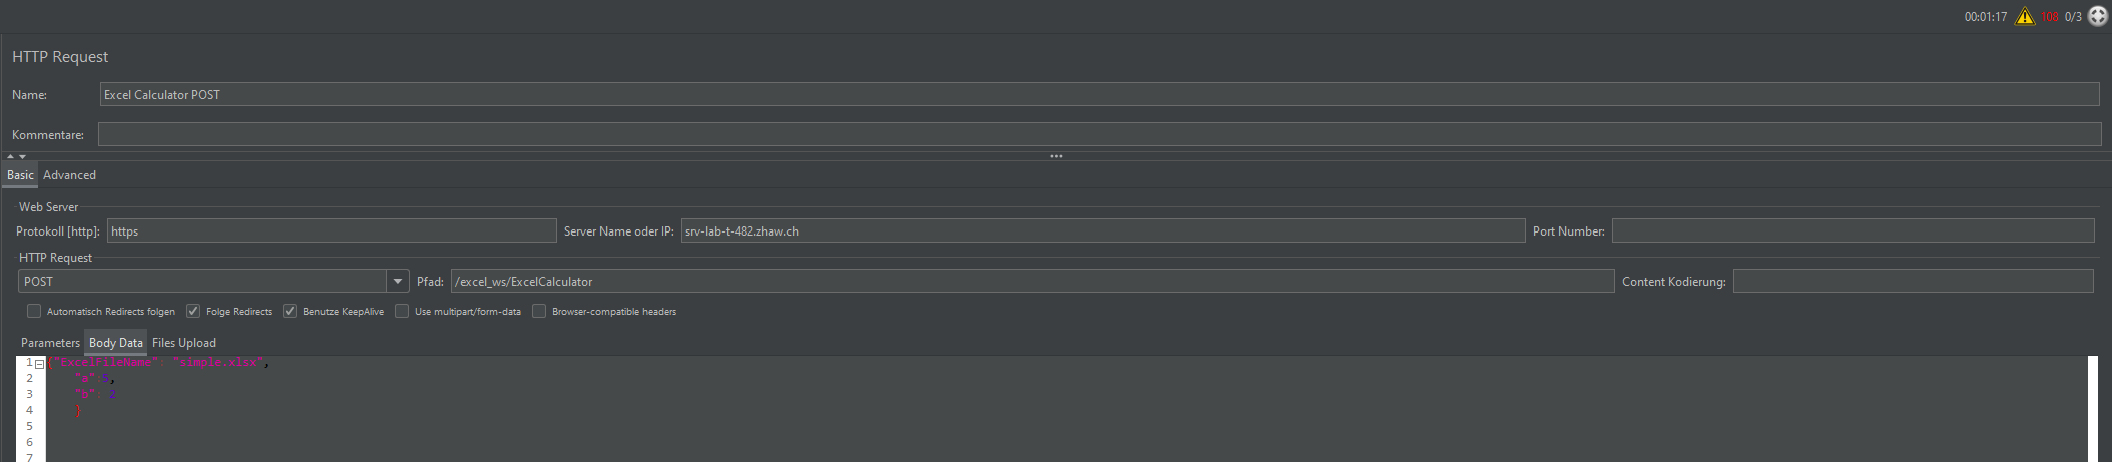
\includegraphics[scale=0.5]{Report/Figures/Formulas Post Request.png}
  \caption{Formulas Post request}
  \label{fig:App registration process}
\end{figure}

 As the addressed server is hosted by zhaw, a VPN connection to ZHAW is needed in order to perform the request. It is further needed to create an HTTP Header Manager which the specifications as shown below. Connection needs to be set to keep-alive so a persistent connection can be kept between requests and a new one will not be initiated on every request. The Accept Attribute is set to */* such that all types of responses are accepted. Content-type is further set to application/Json such that the type of content in the request bodies is specified. \\[0.5cm]

\begin{figure}[h!]
  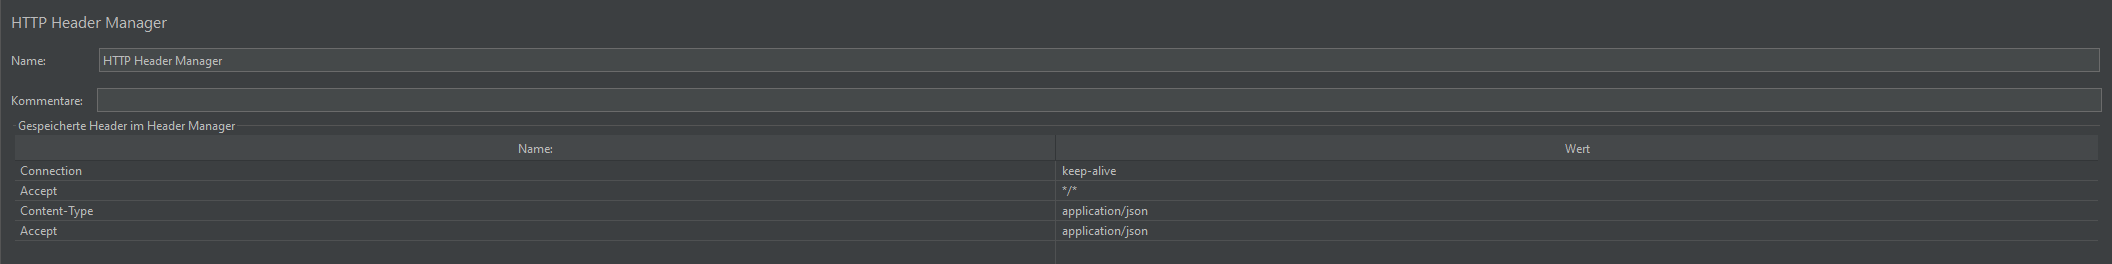
\includegraphics[scale=0.5]{Report/Figures/Http Header Manager.png}
  \caption{Formulas Post request}
  \label{fig: Http Header Manager}
\end{figure}

The key statistics of the result of the performance Test is as shown below. 

\begin{longtable}[]{@{}llllll@{}}
\toprule
Samples & Average & Mean & Min & Max & Std. dev.\tabularnewline
\midrule
\endhead
250 & 314 & 307 & 227 & 665 & 54\tabularnewline
\bottomrule
\caption{Key statisitcs}
\label{Required API permissions}
\end{longtable}

The according box plot:

\begin{figure}[h!]
  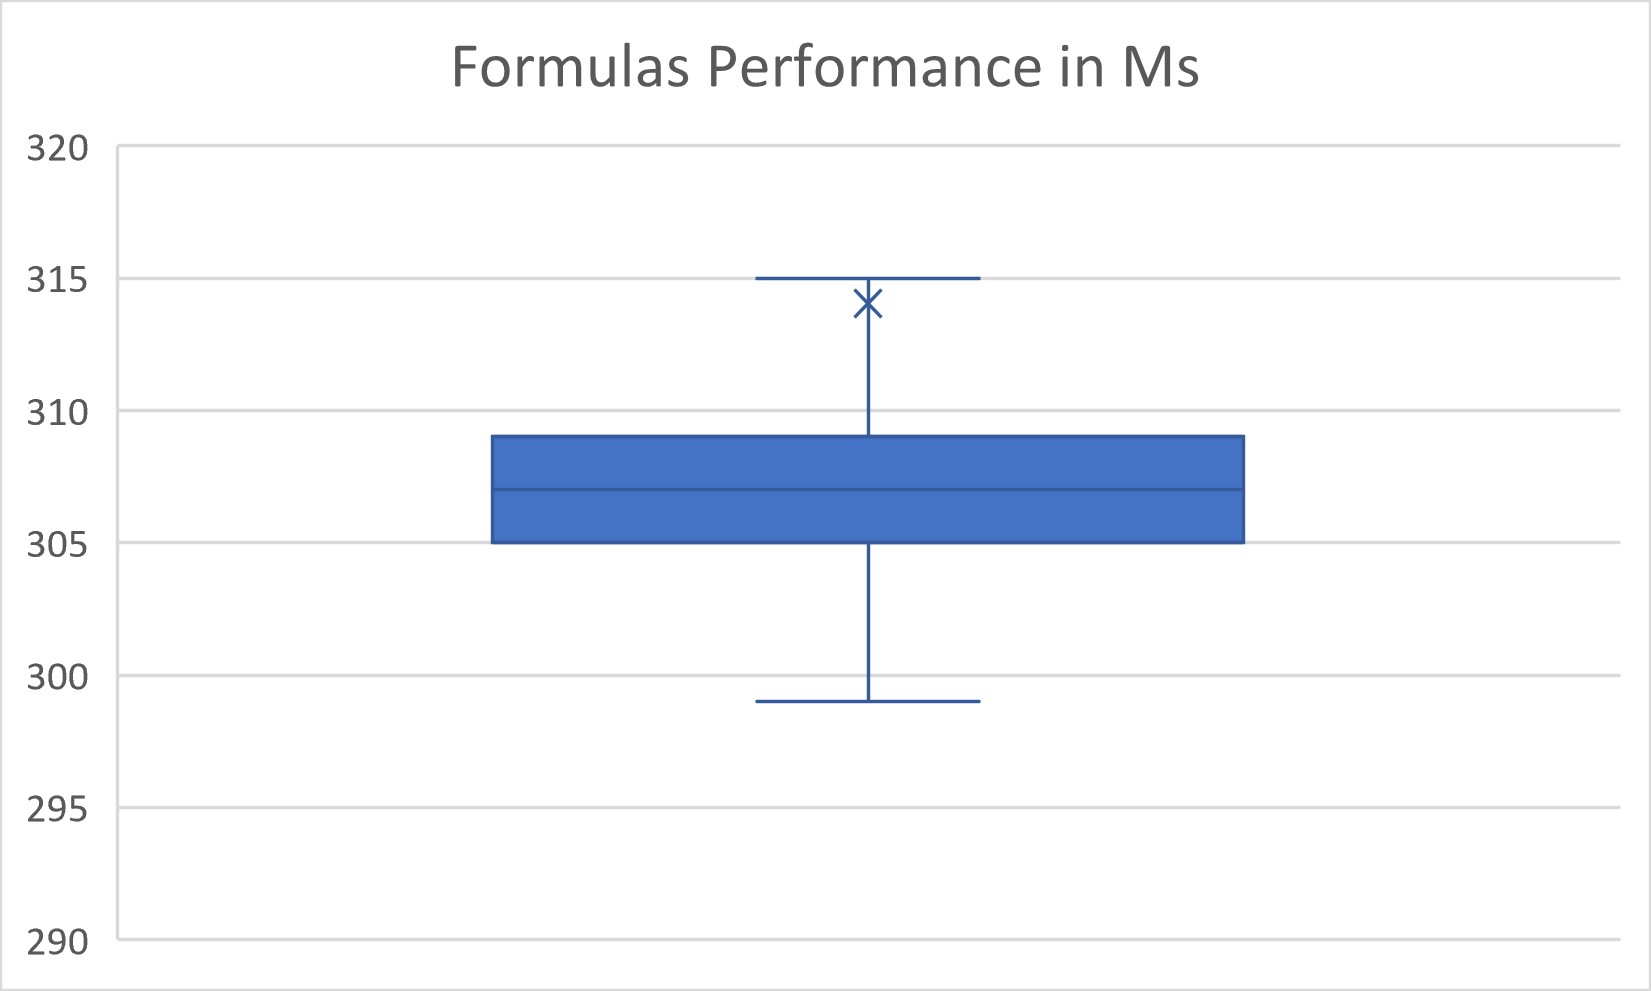
\includegraphics[scale=1]{Report/Figures/Formulas performance.jpg}
  \caption{Formulas performance}
  \label{fig: Formulas performance}
\end{figure}

For the testing of the Graph API, the same actions are performed as in the example before with formulas. As in Graph it is not possible to send the output back to the user in the body of the Post request, it is required to perform at first a Patch request to write the Input data to sheet. Second, it is required to read the Output value which is calculated by the Excel. 

The Patch request which is triggered fist, looks as shown below. The User ID and the Item ID must be specified in the request along with patch to the cells which need to be written. 

\begin{figure}[h!]
  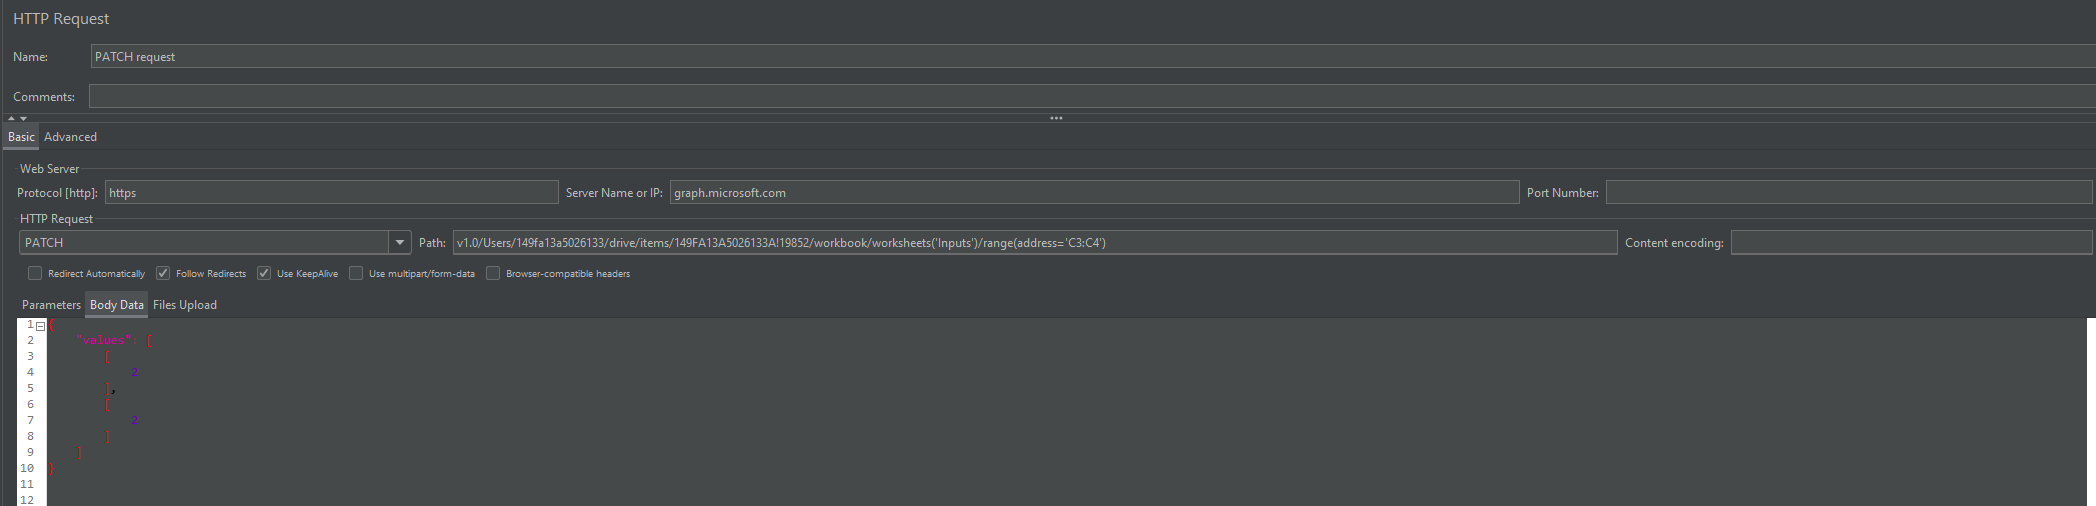
\includegraphics[scale=0.5]{Report/Figures/Graph API Patch request.png}
  \caption{Graph API Patch request}
  \label{fig: Graph API Patch request}
\end{figure}

After the Input data has been written to the Excel, it can be read and displayed as output by the following Get request:

\begin{figure}[h!]
  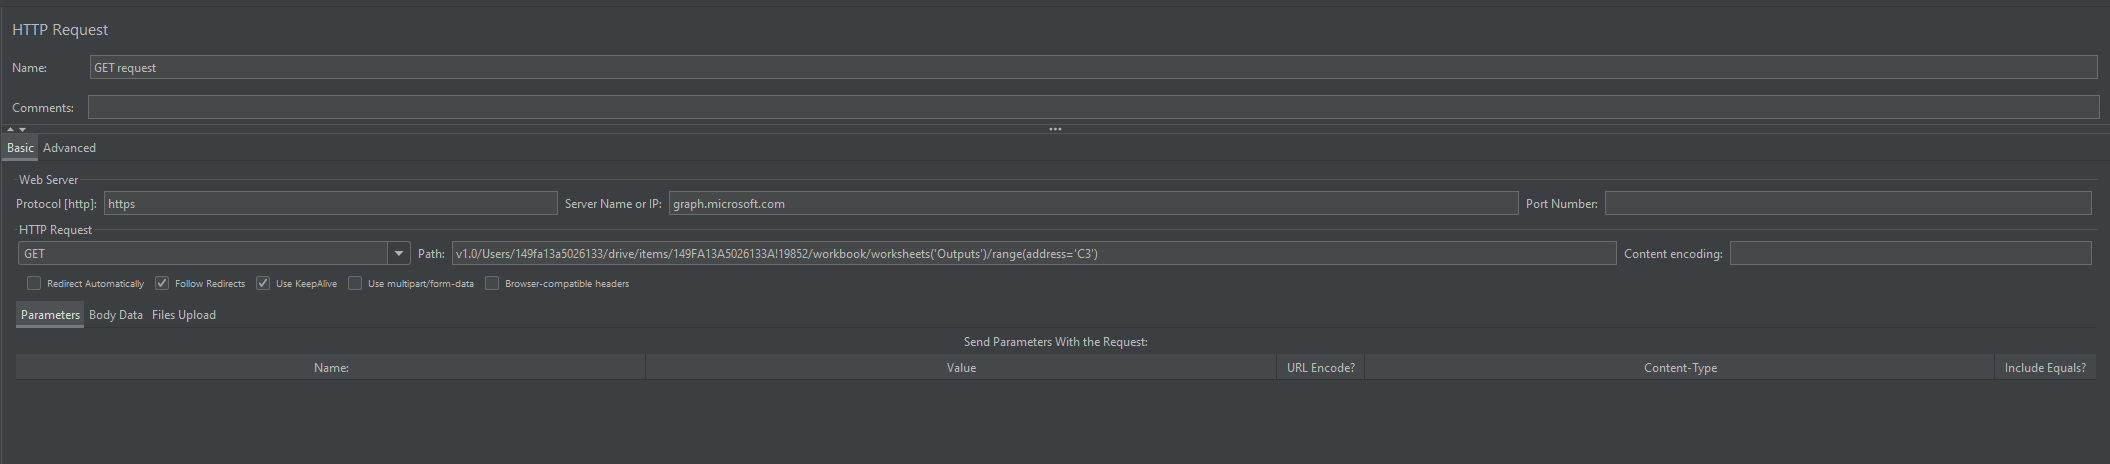
\includegraphics[scale=0.5]{Report/Figures/Graph API Get request.png}
  \caption{Graph API Get request.png}
  \label{fig: Graph API Get request.png}
\end{figure}

Graph API Patch request key statistics:

\begin{longtable}[]{@{}llllll@{}}
\toprule
Samples & Average & Mean & Min & Max & Std. dev.\tabularnewline
\midrule
\endhead
250 & 1940 & 1840 & 306 & 7389 & 1103\tabularnewline
\bottomrule
\caption{Key statistics}
\label{Required API permissions}
\end{longtable}

Graph API Patch request performance

\begin{figure}[h!]
  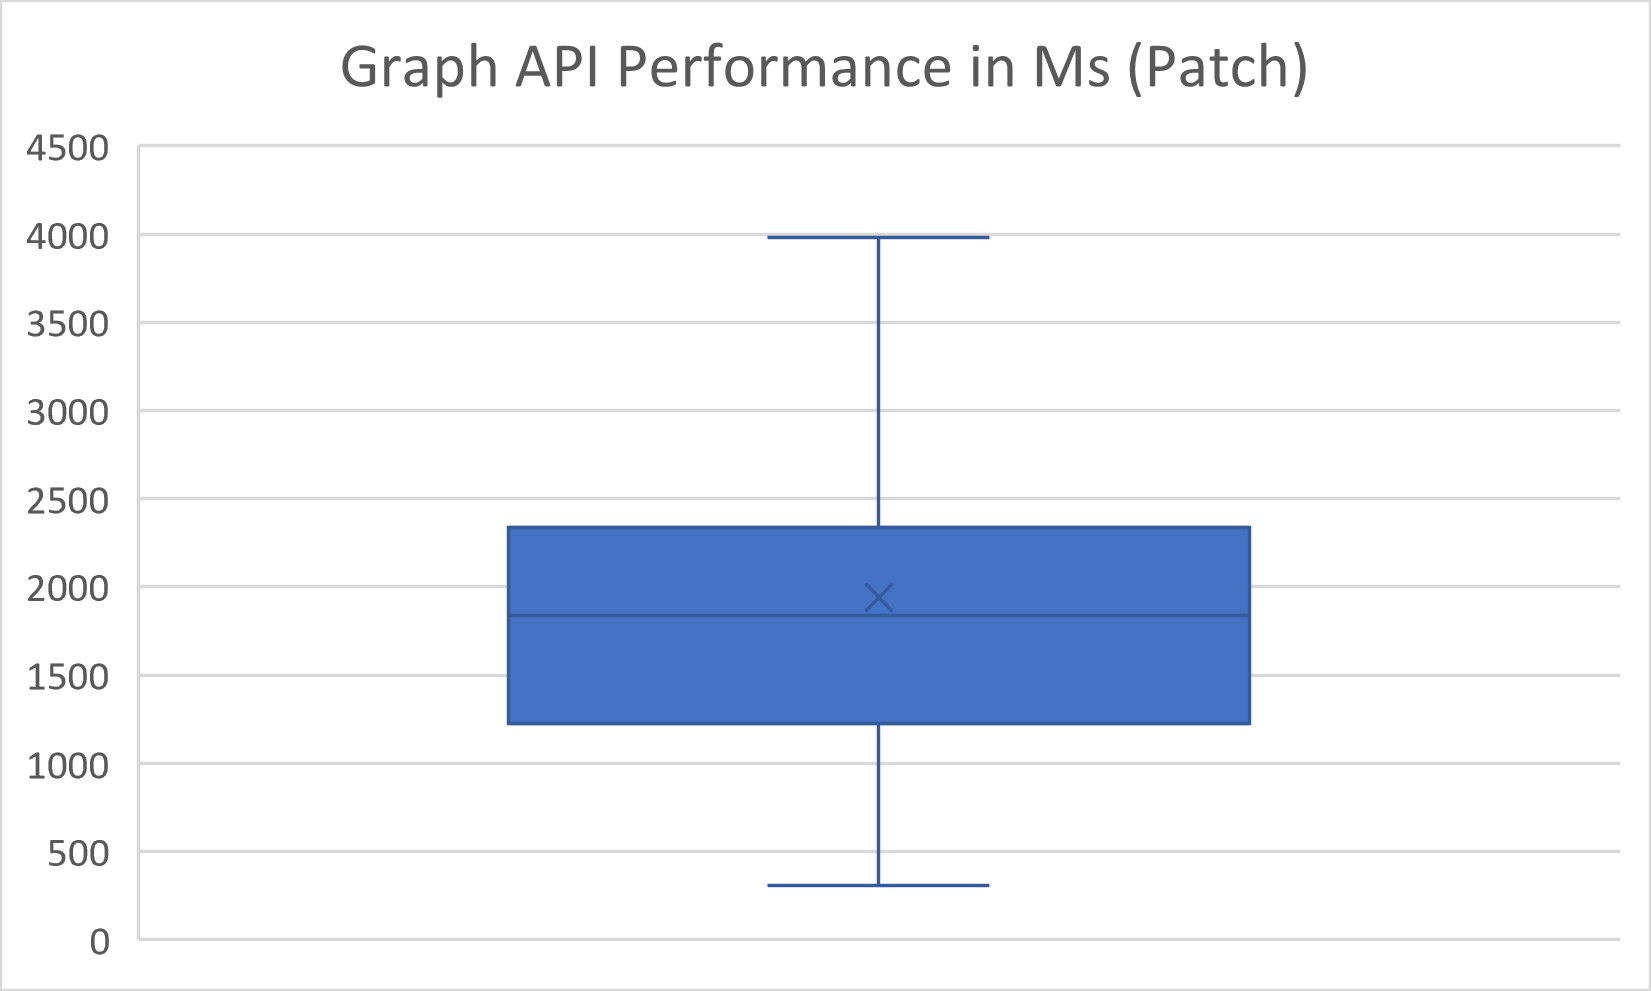
\includegraphics[scale=0.5]{Report/Figures/Graph API Patch request performance.jpg}
  \caption{Graph API Patch request performance}
  \label{fig: Graph API Patch request performance}
\end{figure}


Graph API Get request key statistics:

\begin{longtable}[]{@{}llllll@{}}
\toprule
Samples & Average & Mean & Min & Max & Std. dev.\tabularnewline
\midrule
\endhead
250 & 1089 & 921 & 491 & 11979 & 1039\tabularnewline
\bottomrule
\caption{Key statistics}
\label{Required API permissions}
\end{longtable}

Graph API Get request performance:

\begin{figure}[h!]
  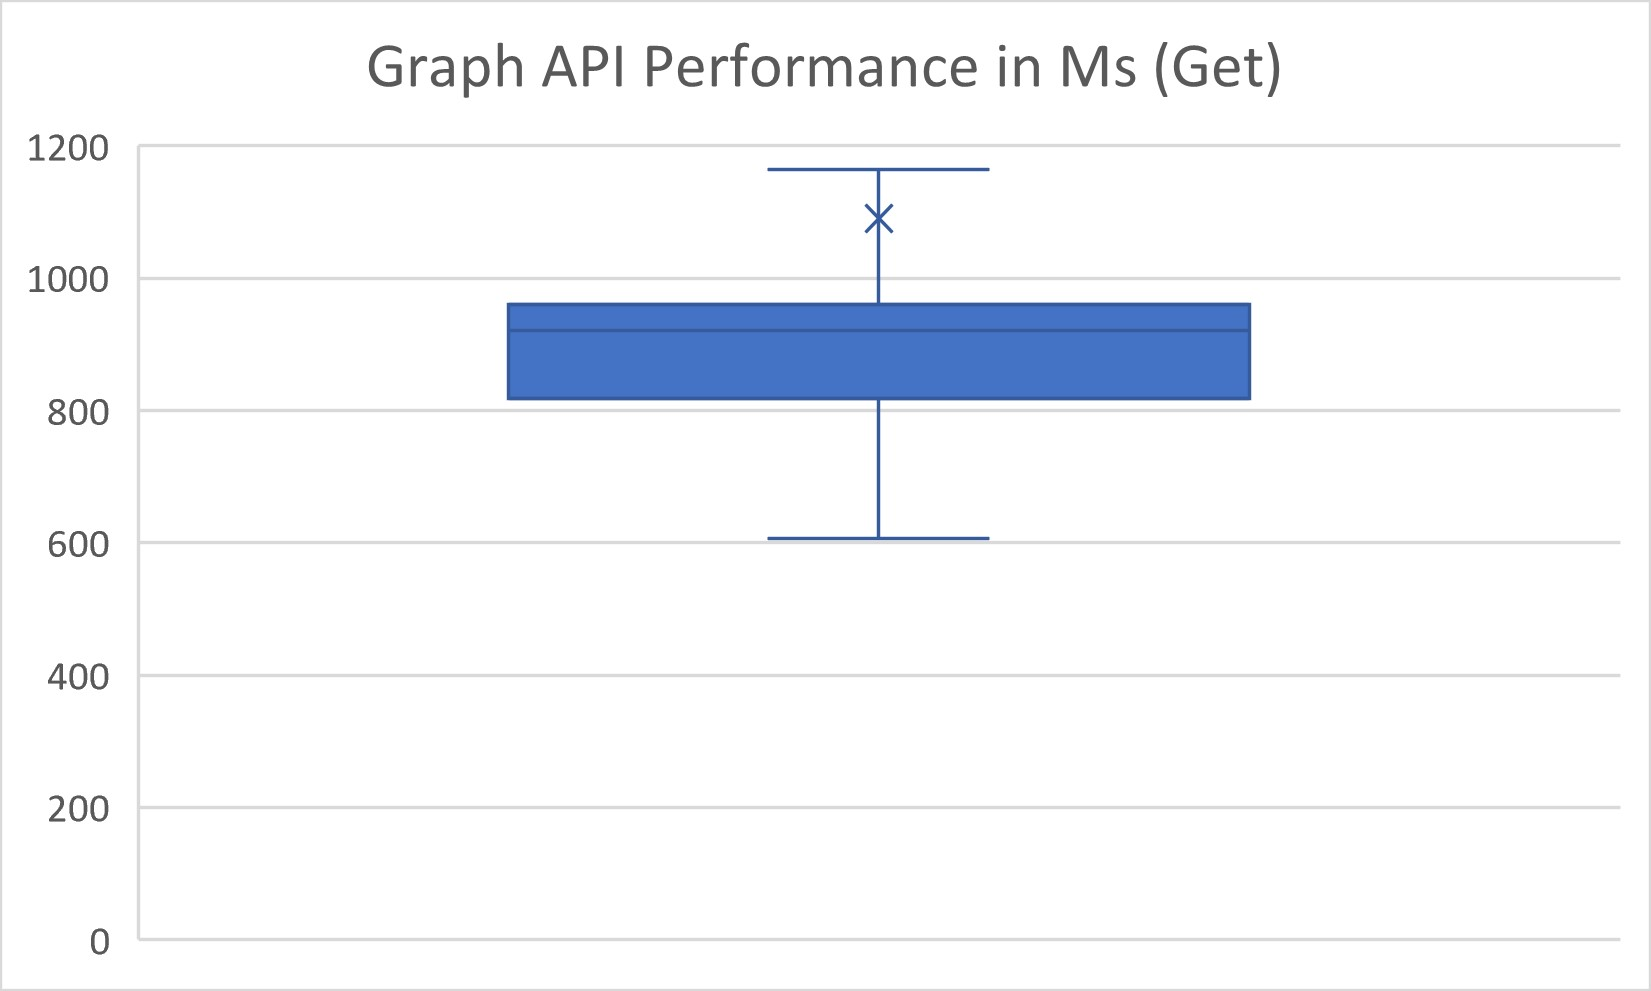
\includegraphics[scale=0.5]{Report/Figures/Graph API Get request performance.jpg}
  \caption{Graph API Get request performance}
  \label{fig: Graph API Get request performance}
\end{figure}















